\subsection{Exercício 3}
Relativamente ao exercício 3, era pedido que se criasse um diagrama de correlação entre todos os atributos.

De facto, este diagrama de correlação é um tipo de exibição de dados que mostra a relação entre duas variáveis numéricas. Assim, e como estes dados têm de ser numéricos, passou-se à observação em detalhe dos dados importados.

Em primeiro lugar, passou-se à atribuição de 0 e 1 aos atributos não numéricos que apenas tinham 2 opções (no caso variavam entre "Sim" e "Não" e "Feminino" e "Masculino"). Em segundo lugar, para os atributos não numéricos com mais de 2 opções, foi utilizada a livraria "fastDummies" com a função "dummy cols" aplicando a técnica "One-Hot Encoding". Assim, para além de variáveis numéricas já existentes, todos os restantes atributos ficaram nesse mesmo tipo. Por fim, alterou-se o nome das colunas dos dados e realizou-se o diagrama de correlação como se verifica na Fig. 3. Devido à enorme quantidade de atributos, o diagrama de correlação segue junto com os scripts em formato pdf de forma a se poder observar melhor.

\begin{figure}[htbp]
\centerline{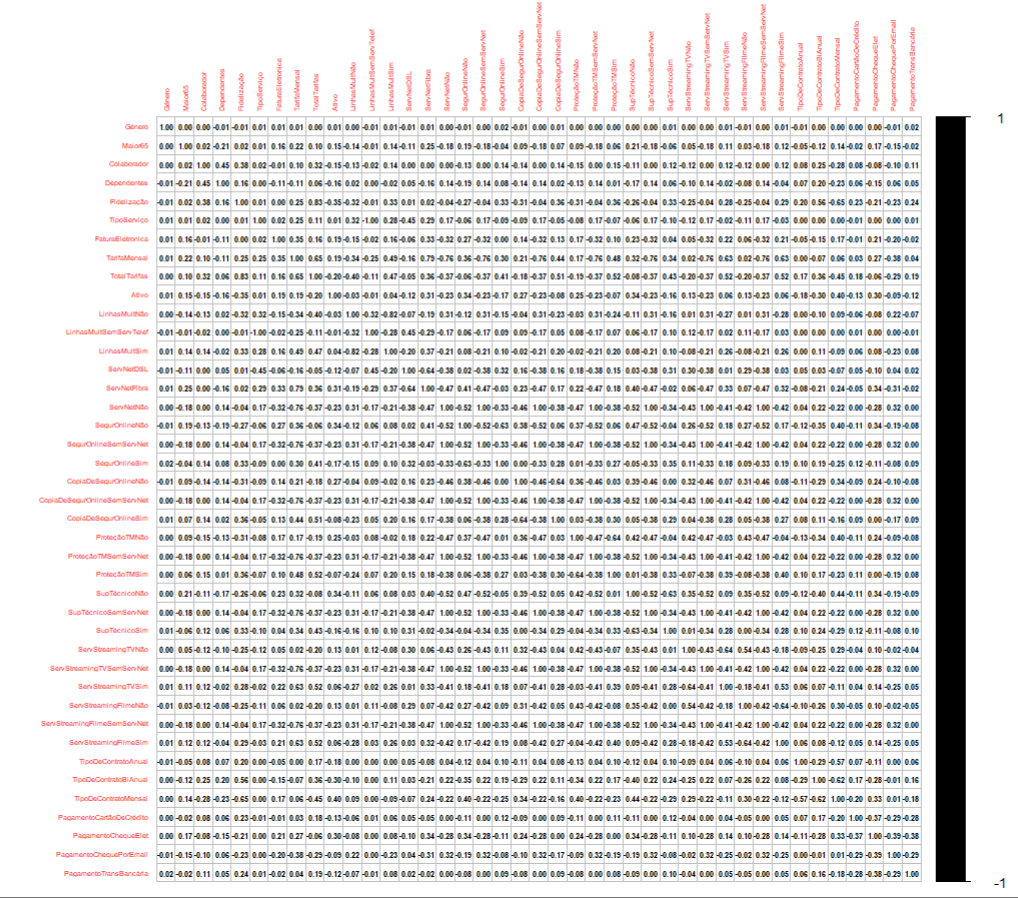
\includegraphics[width=9.5cm]{images/ex3_diagrama_correlacao.png}}
\caption{Diagrama de correlação entre todos os atributos.}
\label{ex3_diagrama_correlacao}
\end{figure}